\chapter{Exploring Bifurcations between Phenotypes}
\label{chapter:exploring}
\begin{music}
    \parindent10mm \instrumentnumber{1} \setstaffs1{1} 
    \generalmeter{\meterfrac44} \generalsignature{2}
    \startextract
            \notes \ql j \ql i \Qqbl ieji \en
        \bar \zw{m*} \bar 
            \notes \ql i \qu h \Qqbu hdih \en
        \bar \zw{l*} 
    \zendextract
\end{music}
\epigraph{\textit{Who knows what might happen to those who are consumed by greed}}{Ocarina of Time}

\section{Preface}
\subsection{Problem Statement \& Context}
The studies in chapters \ref{chapter:double-exclusive}-\ref{chapter:inference} were carried out under the assumption that the underlying microscopic mechanisms that give rise to different phenotypes of an organism are known, and therefore can be modelled with differential equations that have interpretable parameters $\theta$. In section \ref{section:phenotype-inference} we outlined some popular machine learning approaches that can be used in settings where the underlying mechanism is partially or completely unknown. This chapter presents a study in immunology. While detailed models of the immune system exist \cite{}, in the advent of high-throughput biology new mechanisms and exceptions are continuously being discovered \cite{}. This is done by identifying immune cell populations, their function and mechanism of action from tissue and blood samples taken from an organism in homeostasis. \emph{Immunophenotyping} methods use antibodies to identify cells based on the types of antigens or markers on their surface. As we shall see, such datasets are typically high-dimensional data clouds that can be reduced with the help of \emph{universal function approximators} and clustered to identify different immune cell phenotypes. Such high-dimensional data clouds also appear in chapter \ref{chapter:inference} when optimal parameters $\theta$ reveal clusters of topologically or geometrically equivalent models.

In this chapter we argue the importance of interactive tools that allow immunologists to navigate high-dimensional data clouds from heterogeneous experimental setups. Such tools enable crowd-sourced consensus phenotyping of cell populations, discovery of rare populations and iterative refinement of a model of the immune system. An interactive tool \emph{FlowAtlas.jl} is presented in an adaptation of a manuscript prepared for \emph{Nature Methods: Brief Communications} at the time of writing the thesis. While the focus of this chapter remained grounded in immunology, we note these methods can be adapted to multi-omics data \cite{}. We conclude this chapter with a vision of how approaches in chapters \ref{chapter:inference} and \ref{chapter:exploring} can be combined to realise a high-throughput \emph{Design-Learn} pipeline.

\subsection{Contributions}
\textbf{Grisha Szep} is co-first author with \textbf{Valerie Coppard}. \textbf{Joanne Jones}, \textbf{Daniel Rainbow}, \textbf{Sarah Howlett} and \textbf{Lorna Jarvis} conceived and designed the study. \textbf{[missing name]} processed donor tissue samples. \textbf{Valerie Coppard} designed the flow cytometry panels and performed the experiments. \textbf{Grisha Szep} conceived and implemented computational pipeline and interactive software. All authors analysed and interpreted the data. \textbf{Grisha Szep} and \textbf{Valerie Coppard} wrote the main text. All authors provided input into the manuscript.
\clearpage

\section{Abstract}
\noindent As the dimensionality, throughput and complexity of cytometry data increases, so does the demand for user-friendly, interactive analysis tools that leverage high-performance machine learning frameworks. We introduce FlowAtlas.jl: an interactive web application that bridges the familiar user-friendly environment of FlowJo and computational tools in Julia developed by the rapidly growing scientific machine learning community. We demonstrate the workflow on a novel human multi-tissue, multi-donor dataset, addressing relevant biological questions with examples.

\section{Introduction}
Rapid advancements in the capabilities of flow and mass cytometry have brought about a new era of high-dimensional cell phenotyping. Modern cytometers allow unprecedented ability to measure over 40 parameters \cite{Park2020OMIP-069:Blood} and the pace of multi-parametric analyses as well as the development of new dyes, with improved spectral performance, has been accelerating in recent years. However, these technological advancements have not been accompanied by equally impressive developments in user-friendly data analysis tools necessary to deliver a powerful, intuitive and unbiased approach to the analysis of high-dimensional data. At present, exploratory analysis of multi-parametric data presents researchers with a considerable challenge. The widely used commercial platforms such as FlowJo rely on manual sequential cell population gating, best suited for targeted analyses of well-defined cell subsets, rather than exploratory discovery of novel populations in high-complexity datasets. Although an attempt has been made to integrate dimensionality reduction and automated cell population clustering algorithms into these platforms, the algorithm implementations lack flexibility and interactivity and require substantial data down-sampling, ultimately reducing their utility.

To address the need for computational tools designed specifically for data discovery, exploration and visualisation, a number of stand-alone computational pipelines written in R, Matlab and Python programming languages have been developed. However, despite their advanced capabilities, uptake amongst biomedical researchers remains low - most likely due to the lack of inter-operability with familiar tools such as FlowJo, as well as high entry requirements for computational literacy.

\begin{Figure}
    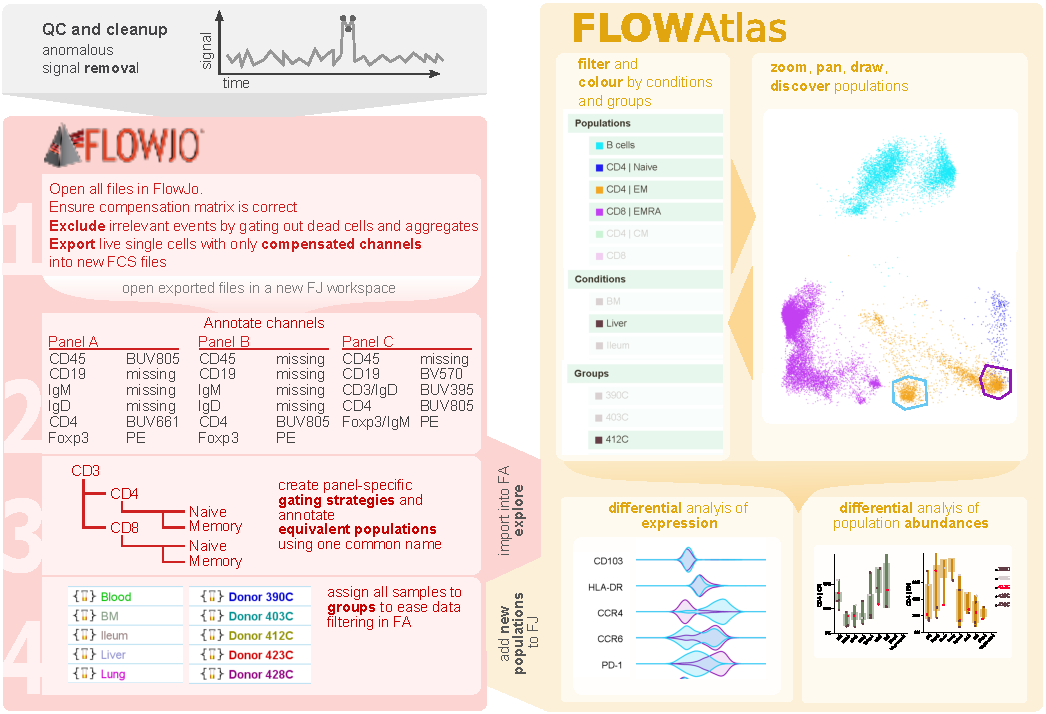
\includegraphics[width=12cm]{overview}
    \caption{Overview of FlowAtlas.jl workflow in tandem with FlowJo}
    \label{fig:overview}
\end{Figure}

Here, we present FlowAtlas.jl --- our effort to address the growing need for high-performance, flexible and interactive analysis tools that enable the visual, exploration and profiling of hundreds of millions of cells in high-dimensional flow cytometry datasets with no data downsampling or command line input. FlowAtlas.jl is fully inter-operable with FlowJo, allows concomitant analysis of datasets created with non-identical panel designs and empowers researchers to explore data in a fully interactive, graphical environment using a new analysis concept.
We showcase the capabilities of FlowAtlas.jl using a novel, human flow cytometric dataset, consisting of immune cells extracted from the tissues of five deceased organ donors, collected over a 5-month period and stained using three slightly different antibody panels. 

This work is presented in an effort to strengthen the open-source collaborations between researchers using flow cytometry and the rapidly growing scientific machine learning community in Julia programming language.

\section{Proposed Method}
FlowAtlas.jl is designed to be used in an iterative discovery loop with FlowJo, where traditional gating strategies created in FlowJo provide initial annotation of main populations, conditions, and sample filtering options to guide the discovery of new sub-populations in FlowAtlas.jl, inside and outside of the specified gates. To prevent the need for downsampling, we implemented \textit{EmbedSOM} \cite{Kratochvil2018RapidEmbedSOM} a powerful dimensionality reduction method. State-of-the-art missing value handling methods and novel features within FlowAtlas.jl also allow users to merge flow cytometry datasets acquired using different antibody panels enabling their concomitant analysis. For example, in our dataset three  panel designs were used (see Table \ref{table:panels}), where CD4 was assigned to BUV661 in Panel A and to BUV805 in Panels B and C. In addition, Panel C had three B cell makers not present in Panels A or B, whereas Panel A had CD45 which was not present in Panels B and C. Consequently, three panel-specific gating strategies were created in FlowJo (see Extended Figure \ref{fig:gating}) to define common cell populations. FlowAtlas.jl was then able to seamlessly merge these datasets using channel marker annotations provided by the user in FlowJo, and combine equivalent cell populations based on their annotations irrespective of panel-specific gating strategy. Analysis steps are outlined in Figure \ref{fig:overview}.

\subsection{Pre-processing}
Prior to commencing data analysis, we strongly recommend performing raw data QC and clean up. This is necessary to ensure that acquisition anomalies which often result from sudden flow rate or signal acquisition instability are detected and removed (Figure \ref{fig:overview}, top grey box). We performed data clean-up using the interactive implementation of FlowAI \cite{GianniMonaco2017FlowAI}. This will ensure more accurate and reproducible embedding and analysis results. High quality files were saved and imported into FlowJo for next steps of data pre-processing described below.

Next, the cleaned-up files of all datasets to be analysed are imported into FlowJo. Ensure that compensation matrices of every dataset are correct and create simple gating to exclude dead cells and aggregates (Figure \ref{fig:overview} FlowJo box, step 1). Following this, we exported terminal live lymphocyte gate in all samples as new FCS files with only compensated fluorescence channels (leaving our scatter channels). Since data embedding is the most computationally intensive step, removal of irrelevant events reduces file size by approximately 40\% and results in a substantially shortened embedding times without compromising relevant data. From now on, all analysis is performed with these newly exported files.

\subsection{Annotation in FlowJo}

standard hierarchical gating of high-level cell subsets. Samples acquired with different panel designs should be imported into the same FlowJo workspace but separated into different groups and gated with group-specific gating strategy. The goal is to implement panel-appropriate gating, while defining common cell subsets across all sample groups. It is critical to label equivalent populations across all datasets with a common name irrespective of gating strategy that defines them as they are automatically imported into FlowAtlas.jl and used for all further analysis. For example, CD4 effector memory (CD4EM) T cells can be gated differently depending on panel design as illustrated in our dataset see Extended Figure \ref{fig:gating} but they should be labelled as CD4EM in every panel.  In order to ensure successful panel merging by FlowAtlas.jl, all fluorescent channels must also be annotated with their respective markers in FlowJo. Although panel merging precludes differential analysis of expression densities using MFI values for non-identical panels, it still allows qualitative and cell frequency comparisons of common populations across such datasets.

\begin{Figure}
    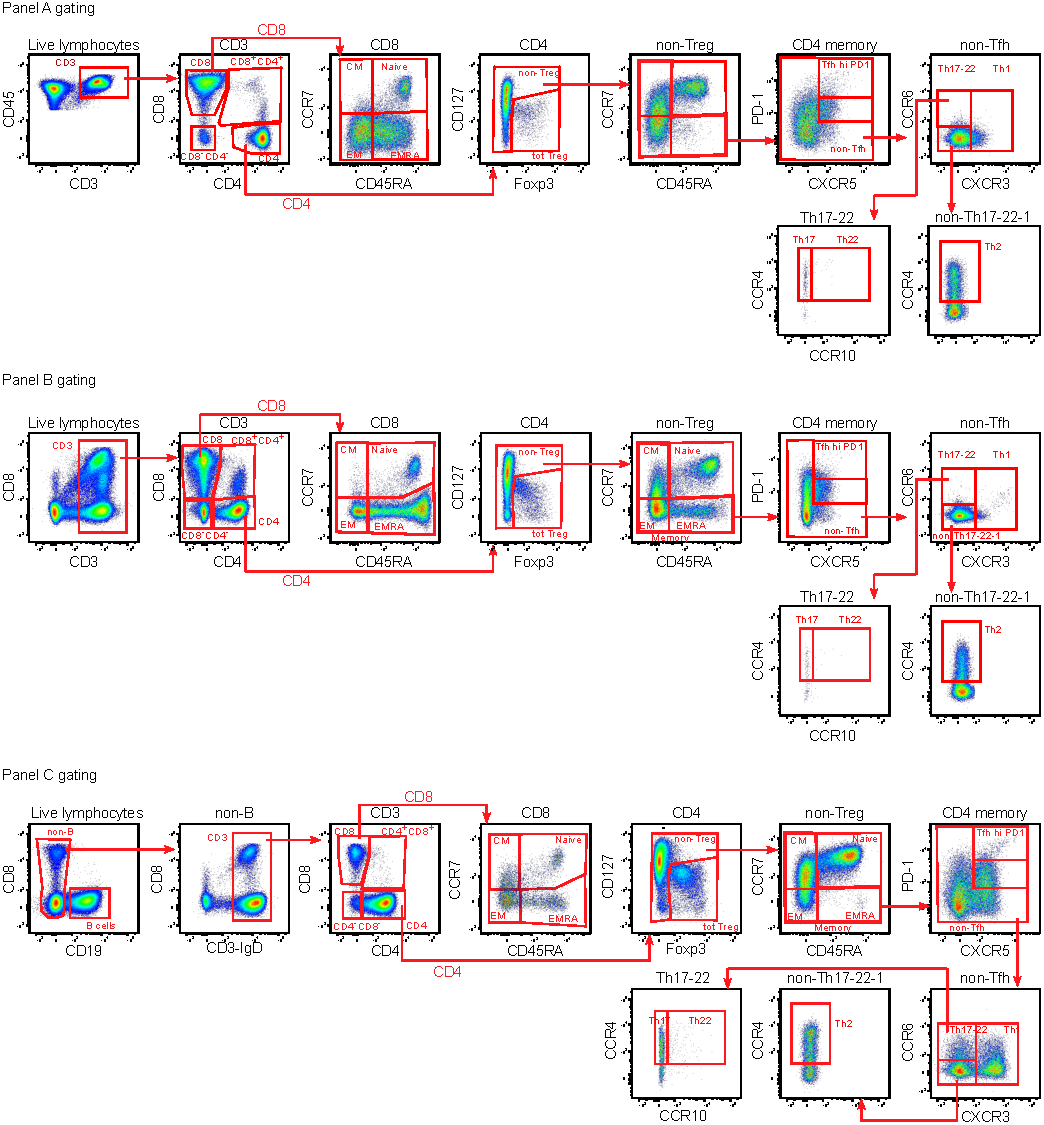
\includegraphics[width=12cm]{Extended_Fig_gating.pdf}
    \caption{Panel-specific gating strategies created in FlowJo.}
    \label{fig:gating}
\end{Figure}

Next, to enable a flexible and intuitive data exploration, group all samples into as many groups as would be informative for exploratory analysis (for example group samples by donor, tissue, treatment, panel, etc). FlowAtlas.jl imports these gate names to population labels without requiring the gating strategies to be the same across different samples and allowing comparative analysis of these populations across datasets. Cells that fall outside of FlowJo-defined gates will be automatically placed into the "Unlabelled" population by FlowAtlas and can be fully explored.

\subsection{Exploration in FlowAtlas.jl}

Next, import FlowJo analysis workspace file (.wsp extension) into FlowAtlas.jl, which will trigger automatic dataset merging and calculation of embedding (Figure \ref{fig:overview}, FlowAtlas box). The embedding computation is performed only once and the embedding file with .som extension is stored in the FlowAtlas.jl folder. This file stores the topology of computed clusters and allows users to quickly return to their analysis. Sharing a .som file together with .wsp and .FCS files with colleagues will allow everyone to work on the same embedding topology and easily confirm findings and analysis reproducibility. Once the computation is complete, FlowAtlas.jl will open a graphical analysis environment in your default browser (Figure \ref{fig:overview}, FlowAtlas box).
We leverage high-performance library GigaSOM.jl \cite{Kratochvil2020GigaSOM.jl:Datasets} and interactive visualisation libraries D3.js \cite{2011D3.js} and OpenLayers \cite{2006OpenLayers} to make the embedding fully interactive, with zooming, panning, event filtering and colouring by marker expression densities or any custom condition (such as sample group) provided by the researcher in FlowJo and where unlimited number of areas of interest (AOI) can be drawn directly in the data embedding for comparative analysis of marker expression with violin plots or comparative frequency analysis of selected cell populations and conditions using box plots. 
For example, Figure \ref{fig:overview} (FlowAtlas box) shows how selecting B cells and CD4 T cell subsets in Liver of donor 412C will display embedding of only cells defined and colour-coded by these filters and allow users to easily identify fine differences in the underlying sub-cluster structures. Any number of such sub-clusters can be interactively compared to each other by drawing colour-coded AOI directly in the embedding and displaying overlayed violin plots of sub-cluster-specific marker expression. Once unique sub-populations are identified, they can be validated in FlowJo where new population gates defining these cells can be created. The new populations will then be read by FlowAtlas,jl and statistics output can be created or further exploration performed. The gating strategy in FlowJo can thus be iteratively updated with new Cell populations discovered in FlowAtlas.jl. The iterative discovery process simplifies the identification of rare or novel cell populations that would otherwise be missed due to data down-sampling or under-fitting in unsupervised clustering approaches.

\section{Results}

\subsection{T-regulatory Sub-populations}
We used total CD4 Treg population (defined in Figure \ref{fig:gating}) to illustrate how new sub-populations can be easily and intuitively identified in FlowAtlas.jl (Figure \ref{fig:tregs}). First, relative population frequency boxplot statistics can be generated for total Treg population across all tissues and panels (Figure \ref{fig:tregs}a). The statistics is calculated relative to the top-level parental population selected in the FlowAtlas.jl or relative to a sum of all selected populations. In our dataset, total Treg represented over 20\% of CD4 T cells in mesenteric lymph nodes in all donors.
Displaying the embedding of total Treg cells for all donors and tissues of Panel C and colouring cells by density of Helios expression (Figure \ref{fig:tregs}b) shows that total Treg population is comprised of Helios\textsuperscript{+} and Helios\textsuperscript{-} sub-populations. Zooming into the embedding reveals additional sub-cluster structures that warrant exploration. Before any further analysis, batch effects that arise due to inter-experimental or inter-panel variability can be easily detected by colouring a cell population by its panel or experiment of origin and observing differences in cluster position, geometry and marker MFI as we did for tot Treg in Figure \ref{fig:tregs}c. Note how CD4 MFI creates a bimodal distribution due to different fluorochrome used in Panel A. Although some differences in cluster locations are notable between panels, overall Treg population embedding looks consistent. Next, we used Panel C as a reference for further exploration of sub-cluster characteristics. Once they are defined, same results can be obtained for Panels A and B (Extended Figure is coming). For this, we re-coloured tot Treg embedding shown in b, by tissue origin, drew AOI around individual sub-clusters and inspected the differences in marker expression using auto-generated violin plots (Figure \ref{fig:tregs}d). This showed a clear difference in the expression of CD45RA, CCR7, CCR4 and CD69 between individual AOI, with red having a naive phenotype CD45RA\textsuperscript{+}CCR7\textsuperscript{+}CCR4\textsuperscript{-}CD69\textsuperscript{-}, while yellow, grey and violet showing characteristics of memory subset.
Yellow CD45RA\textsuperscript{-}CCR7\textsuperscript{-}CCR4\textsuperscript{+}CD69\textsuperscript{-}
Grey CD45RA\textsuperscript{-/lo}CCR7\textsuperscript{-}CCR4\textsuperscript{-}CD69\textsuperscript{+} and violet CD45RA\textsuperscript{-}CCR7\textsuperscript{-}CCR4\textsuperscript{+}CD69\textsuperscript{+}. Grey and yellow memory subsets are D69\textsuperscript{+ } - a sign of tissue homing. Dividing the embedding by tissue reveals differences in tissue specific enrichment of individual Treg subsets. With blood lacking the grey and violet subsets, which is in line with their tissue homing phenotype. Next, we validated the presence of these subsets in FlowJo (Figure \ref{fig:tregs}e). Plotting CD69 vs CCR4 for tot Treg subset in thoracic lymph nodes (tLN) clearly shows the presence of the four sub-populations identified in FlowAtlas.jl. We created new FlowJo gates corresponding to the four subsets and returned to FlowAtlas.jl where we re-coloured Treg embedding by these subsets. This revealed that each individual subset includes both Helios\textsuperscript{+} and Helios\textsuperscript{-} sub-populations (refer to the density of Helios expression shown in b). Since FJ gates for the four new Treg subsets have been gated and read by FA, population frequency statistics can be automatically generated (box plots).

\begin{Figure}
    \includegraphics[width=14cm]{Main-figure-2.pdf}
    \caption{Treg sub-population discovery with FlowAtlas.jl and verification with FlowJo}
    \label{fig:tregs}
\end{Figure}

\subsection{T-helper cell populations}

\begin{Figure}
    \includegraphics[width=14cm]{Extended_Th1.pdf}
    \caption{Exploration of Th1 T cell subpopulations.}
    \label{fig:Extended_Th1}
\end{Figure}

\section{Discussion}
FlowAtlas.jl brings new analysis concept to biomedical scientist by linking the familiar FlowJo workflow with high-performance machine learning framework in a fully graphical, interactive environment. FlowAtlas.jl allows an embedding of millions of high-dimensional events to be rapidly computed without downsampling on an average laptop. Moreover, we utilise state-of-the-art missing data handling methods that allow users to perform concomitant cross-study analysis of datasets with non-identical panel designs or marker numbers. The resulting embedding is highly interactive offering zooming to explore deeper cluster structures, colouring events by custom conditions, selectively filtering embedded events by samples or population subsets, generating frequency statistics and drawing AOI directly in the embedding for comparative analysis of marker expression in sub-cluster structures. Findings can be immediately validated in FlowJo in an iterative discovery loop with FlowAtlas.jl simplifying the identification and validation of rare or novel cell populations that would otherwise be missed due to data down-sampling or under-fitting in unsupervised clustering approaches.

\section{Methods}

\subsection{Tissue Acquisition \& Dissociation} 

All samples were collected via the \href{https://www.cbtm.group.cam.ac.uk}{Cambridge Biorepository for Translational Medicine} under Research Ethics Committee approval 15/EE/0152. Tissue was obtained from five deceased organ donors following circulatory death. Donor metadata is given in Extended Data Table \ref{table:donors}. Briefly, following cessation of circulatory function donors proceeded to organ donation. Organs were perfused \emph{in situ} with cold organ preservation solution and cooled with topical application of ice. Samples for the study were obtained within 60 minutes of cessation of circulation and placed in University of Wisconsin organ preservation solution for transport at 4°C to the laboratory. Lung and liver samples were obtained from the left lower lobe of the lung and the right lobe of the liver. In addition, two donor-matched blood samples were collected prior to withdrawal of life support, under approval 97/290.

To minimise the possibility of processing-depended differences in cell surface marker expression, all samples, including blood, were processed using enzymatic digestion protocol. Briefly, solid tissues were weighed, transferred into 10cm tissue culture dishes and cut into small pieces. Up to 5g of tissue was then transferred to each of eight GentleMACS C tubes (Miltenyi Biotec) containing 5mL of dissociation media composed of X-vivo15 supplemented with 0.13U/mL Liberase TL (Roche), 10U/mL Benzonase nuclease (Millipore/Merck), 2\% (v/v) heat-inactivated fetal bovine serum (FBS, Gibco), penicillin (100 U/ml, Sigma-Aldrich), streptomycin (0.1 mg/ml, Sigma-Aldrich), and 10mM HEPES (Sigma Aldrich). The samples were then dissociated on a GentleMACS Octo dissociator (Miltenyi Biotec) running a protocol that provided gradual ramping up of homogenisation speed and two 15 minute heating/mixing steps at 37°C. Digested tissue was passed through a 70$\mu$m MACS Smartstrainer (Miltenyi Biotec) and the flow-through was first washed with media supplemented with 2 mM EDTA and then with PBS. Mononuclear cells were enriched by Ficoll-Paque (GE Healthcare) density centrifugation according to manufacturer's instructions. Following, density centrifugation, mononuclear layer was collected, washed once with PBS and cell pellet was resuspended in FACS buffer (PBS, 2.5$\%$ FBS).

Bone marrow aspirates and peripheral blood samples were first subjected to Ficoll-Paque density centrifugation, according to manufacturer's instructions, the mononuclear layer was then collected, washed with PBS and cells were treated with the same dissociation media as solid tissues for 30 min at 37°C prior to washing and resuspension in FACS buffer.

\subsection{Flow Cytometry}

Depending on the cell yield, up to 1x10\textsuperscript{6} mononuclear cells/tissue were stained with antibodies shown in Extended Data Table \ref{table:panel}. Not all donors were stained with the same panel. To expand total number of markers, sentinel panel design was implemented where CD3 and IgD were detected with antibodies conjugated to BUV395 and Foxp3 and IgM were detected with antibodies conjugated to PE in some donors. Refer to Extended Data Table \ref{table:panels} for details. 

Single cell suspensions were washed once in PBS, transferred into 96 v-bottom plate and stained with Zombie UV viability dye for 30 min at 4°C following by a wash with FACS buffer. Cell pellets were resuspended in 50$\mu$l FACS buffer with Human FcR block (BD Biosciences) and incubated for 10 min at 4°C. Next, cells were pelleted, excess buffer removed and 100$\mu$l of antibody master mix composed of cell-surface antibody cocktail (see Table Extended Data \ref{table:panels}), BV buffer (BD) and True-Stain Monocyte Blocker (Biolegend) and incubated for 1h at 4°C. Following incubation, cells were washed three times in PBS and prepared for intracellular staining using transcription factor fixation/permeabilisation kit (eBioscience) according to the manufacturer's instructions. Following IC staining, cell were resuspended in PBS and analysed on BD FACSymphony A3 cell analyser within 10 hours.

\subsection{Imputation \& Embedding}

When some markers are not present in every dataset, cells for which a marker is missing are not displayed in the embedding when the embedding is coloured by the expression of the missing marker in FlowAtlas.jl. To compute the initial embedding, however, missing values are sampled from non-missing values. 

or re-use embedding transformations on new datasets. Note that the number of channels and names of the new dataset must match those used to calculate the embedding. With this approach it is possible to calculate an embedding for a sub-sampled dataset to save time and use the resultant transformation on the whole dataset to retain the embedding coordinates of rare populations.
Enables novel population discovery

\subsection{Data \& Code Availability}
All data is made available in \href{https://flowrepository.org}{\texttt{FlowRepository}}. Code and installation instructions can be found in our GitHub \href{https://github.com/gszep/FlowAtlas.jl}{\texttt{github.com/gszep/FlowAtlas.jl}}

\section{Afterword}

% \subsection{Julia \& SciML}
% \subsection{OpenLayers \& Data-driven Documents}
% \subsection{Interactivity}
% \subsection{Dataset Integration}